\renewcommand{\myscale}{.3}
\begin{tikzpicture}[scale=\myscale,inner sep=1pt]
%\draw[help lines,step=1cm] (0,0) grid (12,6);

%Source - like a battery
\node[label=right:$E$] at (0,3)
{{\begin{tikzpicture}[scale=\myscale]
%	\useasboundingbox (-.5,-3) rectangle (.5,3);
	\draw (0,0) circle (1cm);
	\draw (.3,.5) -- (-.3,.5);
	\draw (0,.2) -- (0,.8);
	\draw (.3,-.5) -- (-.3,-.5);
	\draw (0,1) -- (0,3);
	\draw (0,-1) -- (0,-3);
	\end{tikzpicture}
}};

%Resistor
\node[label=right:$R_2$] at (6,3) 
{{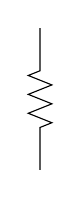
\begin{tikzpicture}[scale=\myscale]
%	\useasboundingbox (0,-3) rectangle (0,3);
	\draw (0,-3) -- ++(0,1.8) -- ++(.5,.2) 
		-- ++(-1,.4) -- ++(1,.4)
		-- ++(-1,.4) -- ++(1,.4)
		-- ++(-1,.4) -- ++(.5,.2)
		-- ++(0,1.8) ;
	\end{tikzpicture}
}};

%Resistor
\node[label=above:$R_1$] at (3,6) 
{{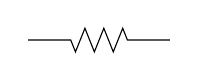
\begin{tikzpicture}[scale=\myscale,rotate=90]
%	\useasboundingbox (0,-3) rectangle (0,3);
	\draw (0,-3) -- ++(0,1.8) -- ++(.5,.2) 
		-- ++(-1,.4) -- ++(1,.4)
		-- ++(-1,.4) -- ++(1,.4)
		-- ++(-1,.4) -- ++(.5,.2)
		-- ++(0,1.8) ;
	\end{tikzpicture}
}};

%Resistor
\node[label=right:$R_3$] at (12,3) 
{{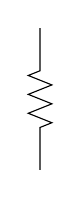
\begin{tikzpicture}[scale=\myscale,rotate=0]
%	\useasboundingbox (0,-3) rectangle (0,3);
	\draw (0,-3) -- ++(0,1.8) -- ++(.5,.2) 
		-- ++(-1,.4) -- ++(1,.4)
		-- ++(-1,.4) -- ++(1,.4)
		-- ++(-1,.4) -- ++(.5,.2)
		-- ++(0,1.8) ;
	\end{tikzpicture}
}};

%Loops
\node[label=above:$L$] at (3,0) 
{{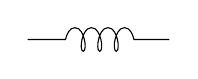
\begin{tikzpicture}[scale=\myscale,rotate=90]
	\useasboundingbox (-.5,-3) rectangle (.5,3);
        \draw (0,-3) -- ++(0,1.5) 
	.. controls+(15:.2) and +(-90:.25) .. ++(.5,.4) 
	.. controls+(90:.25) and +(-15:.2) .. ++(-.5,.4) 
	.. controls+(-15:-.2) and +(90:.1) .. ++(-.5,-.05) 
	.. controls+(-90:.1) and +(15:-.2) .. ++(.5,-.05) 
	.. controls+(15:.2) and +(-90:.25) .. ++(.5,.4) 
	.. controls+(90:.25) and +(-15:.2) .. ++(-.5,.4) 
	.. controls+(-15:-.2) and +(90:.1) .. ++(-.5,-.05) 
	.. controls+(-90:.1) and +(15:-.2) .. ++(.5,-.05) 
	.. controls+(15:.2) and +(-90:.25) .. ++(.5,.4) 
	.. controls+(90:.25) and +(-15:.2) .. ++(-.5,.4) 
	.. controls+(-15:-.2) and +(90:.1) .. ++(-.5,-.05) 
	.. controls+(-90:.1) and +(15:-.2) .. ++(.5,-.05) 
	.. controls+(15:.2) and +(-90:.25) .. ++(.5,.4) 
	.. controls+(90:.25) and +(-15:.2) .. ++(-.5,.4) 
	-- (0,3);
	\end{tikzpicture}
}};



%Capacitor
\node[label=above:$C$] at (9,0) 
{{\begin{tikzpicture}[scale=\myscale,rotate=90]
%	\useasboundingbox (0,-3) rectangle (0,3);
	\draw (0,-3) -- ++(0,2.8) 
		-- ++(.5,0) -- ++(-1,0) 
		++(0,.4) -- ++(1,0)
		-- ++(-.5,0) -- ++(0,2.8);
	\end{tikzpicture}
}};


%Straight Path
%\node at (3,6) 
%{{\begin{tikzpicture}[scale=\myscale,rotate=90]
%	\draw (0,-3) -- (0,3);
%	\end{tikzpicture}
%}};

%Straight Path
\node at (9,6) 
{{\begin{tikzpicture}[scale=\myscale,rotate=90]
	\draw (0,-3) -- (0,3);
	\end{tikzpicture}
}};

%Straight Path
%\node at (9,0) 
%{{\begin{tikzpicture}[scale=\myscale,rotate=90]
%	\draw (0,-3) -- (0,3);
%	\end{tikzpicture}
%}};


%Arrow to represent Current
\node[label=right:$I_1$] at (0,5) 
{{
\begin{tikzpicture}[scale=\myscale,rotate=0]
	\filldraw (0,.4) -- (-.2,-.4) -- (0,-.3) -- (.2,-.4);
	\end{tikzpicture}
}};

%%Arrow to represent Current
%\node[label=above:$i_1$] at (3,6) 
%{{\begin{tikzpicture}[scale=\myscale,rotate=-90]
%	\useasboundingbox (0,-.4) rectangle (0,.4);
%	\filldraw (0,.4) -- (-.2,-.4) -- (0,-.3) -- (.2,-.4);
%	\end{tikzpicture}
%}};

%Arrow to represent Current
\node[label=right:$I_2$] at (6,5) 
{{
\begin{tikzpicture}[scale=\myscale,rotate=180]
%	\useasboundingbox (0,-.4) rectangle (0,.4);
	\filldraw (0,.4) -- (-.2,-.4) -- (0,-.3) -- (.2,-.4);
	\end{tikzpicture}
}};

%Arrow to represent Current
\node[label=above:$I_3$] at (9,6) 
{{
\begin{tikzpicture}[scale=\myscale,rotate=-90]
%	\useasboundingbox (0,-.4) rectangle (0,.4);
	\filldraw (0,.4) -- (-.2,-.4) -- (0,-.3) -- (.2,-.4);
	\end{tikzpicture}
}};

%Node
\node at (6,6) 
{{\begin{tikzpicture}[scale=\myscale,rotate=-90]
%	\useasboundingbox (0,-.4) rectangle (0,.4);
	\filldraw (0,0) circle (.15cm);
	\end{tikzpicture}
}};

%Node
\node at (6,0) 
{{\begin{tikzpicture}[scale=\myscale,rotate=-90]
%	\useasboundingbox (0,-.4) rectangle (0,.4);
	\filldraw (0,0) circle (.15cm);
	\end{tikzpicture}
}};

\end{tikzpicture}
